% !TEX root = ../main.tex

\section{Workload Characterization \& Profiling}
\label{sec:workload_analysis}

This section reports the PyTorchSim results for one SmolVLA action chunk (fp32, batch 1, heuristic mapping) on the NPUs of \cref{tab:npus}. All figures are generated by \texttt{src/p1\_profiling/plots/} from the summary data in \texttt{results/}.

\subsection{GEMM workload}
\label{subsec:wl-gemms}

Vision accounts for 76\% of the 839.6~GFLOP of a chunk (\cref{tab:stages}). The shapes separate the stages: vision streams 1024 tokens through each weight, the VLM 241, and the action expert only 50 rows through large weights. This is the batch-1 weight-streaming pattern, with arithmetic intensity of 26--29~FLOP/B for the expert layers, well below the ridge point of every NPU considered. The expert's 1440 GEMMs move 5.1~GB of operands per chunk, close to the 7.2~GB of the vision encoder, at a sixth of its FLOPs. lerobot also recomputes the cross-attention K/V projections of the fixed prefix in every denoise step (160 GEMMs, 7.9~GFLOP per chunk), which caching would remove. The 28 unique GEMM shapes are the workload of the GEMM-level exploration with SCALE-Sim in the next part.

\subsection{Reference NPU}
\label{subsec:wl-big}

On the big NPU a chunk takes \textbf{105.3~ms}: vision 59.7\%, connector 0.5\%, prefix 7.8\%, denoise 32.0\%. The single-session chunk run agrees with the sum of separately simulated stages within 0.1\%, and with single layers times their multiplicity within 0.4\%: the modelled NPU keeps nothing on chip between kernels, so each layer already pays its own DRAM transport. The chunk moves 21.1~GB of DRAM traffic and the arrays are busy only 15\% of the time.

\begin{figure}[tp]
\centering
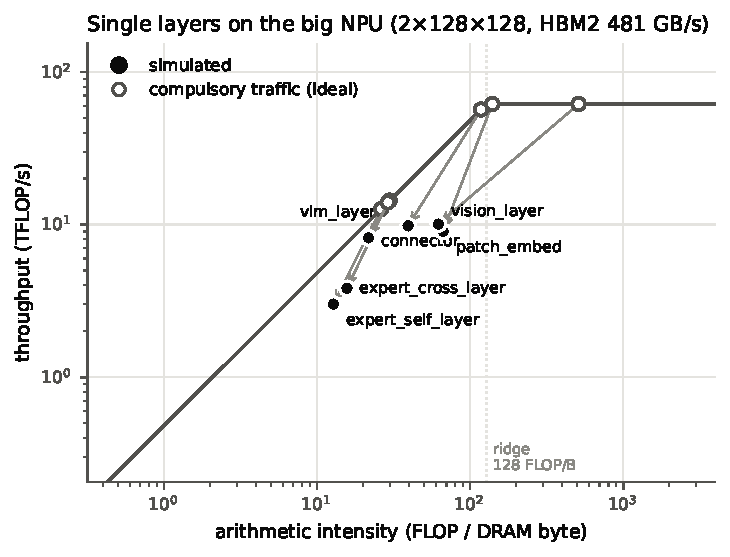
\includegraphics[width=0.55\textwidth]{p1/roofline_layers.pdf}
\caption{Single layers on the big NPU. Filled: simulated; hollow: the same layer with compulsory traffic at its roofline bound.}
\label{fig:roofline-layers}
\end{figure}

\Cref{fig:roofline-layers} places the single layers on the roofline. Every layer reaches only 15--27\% of its bound (the connector 57\%). Vision layers are compute-bound on paper, but move $8\times$ their compulsory traffic; the expert layers are memory-bound by construction. \Cref{subsec:wl-attribution} measures where the time goes: on this NPU the vision stage is 44\% array busy, 33\% vector unit only and 23\% waiting on DRAM, and while it streams the array executes the ideal FLOPs plus only the padding to 128 lanes. The losses are idle array time and extra traffic, not array inefficiency.

\subsection{Edge NPUs}
\label{subsec:wl-edge}

On the edge NPUs a chunk takes \textbf{689~ms} ($64\times64$: vision 60\%, prefix 12\%, denoise 28\%) and \textbf{1030~ms} ($32\times32$: 70 / 8 / 21\%). Going from the big NPU to an edge one shrinks compute (by $8$--$32\times$) and bandwidth (by $9.4\times$) together, and the two act on different stages: vision is limited by compute, the action expert by bandwidth (\cref{subsec:wl-response}). Which stage gains share therefore depends on their ratio, the ridge point. It barely changes from the big NPU to the $64\times64$ one (128 to 160~FLOP/B) and drops to 40 on the $32\times32$ one, so on these two edge NPUs time does not shift towards the action expert. \Cref{fig:kernels} shows the detail: the vector unit shrinks with the array, so the vision flash attention (its softmax runs on the vector unit) grows to a third of the chunk on $32\times32$, while on $64\times64$ the linear-layer GEMMs dominate (59\%). Prefix and denoise run at 85--90\% of the LPDDR5 peak on both edge NPUs. The sweeps below vary bandwidth and array size one at a time.

\begin{figure}[tp]
\centering
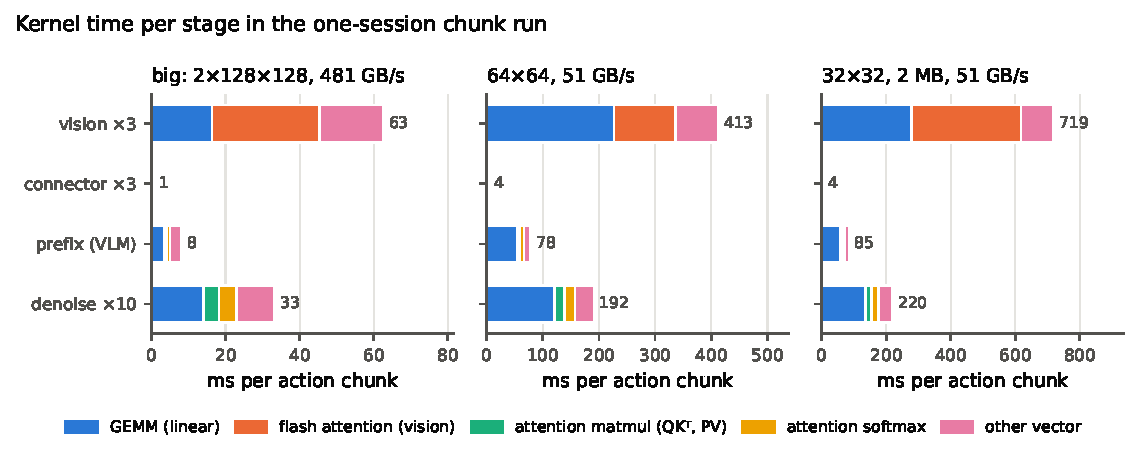
\includegraphics[width=\textwidth]{p1/kernel_classes.pdf}
\caption{Time per stage and kernel type inside the one-session chunk run (per chunk, i.e.\ including the $3\times$ and $10\times$ repetitions).}
\label{fig:kernels}
\vspace{1.5em}
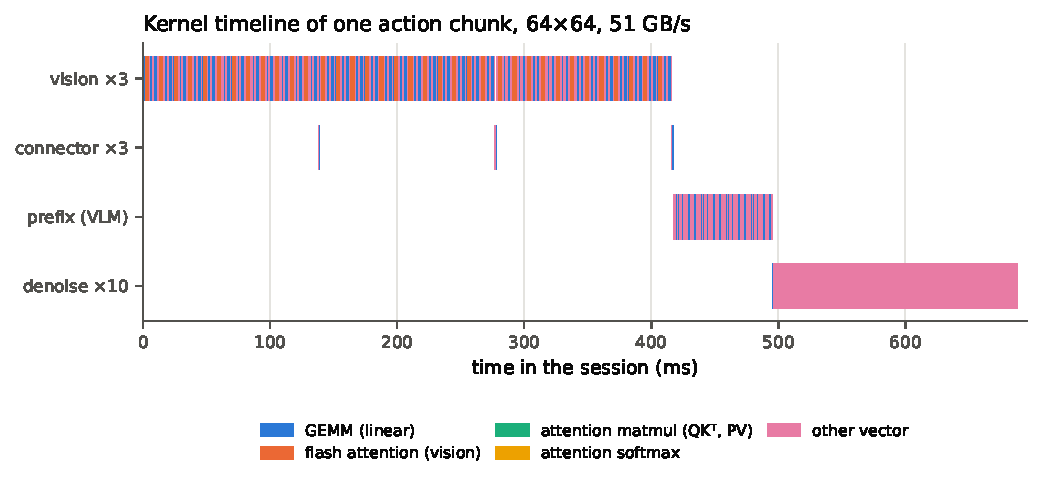
\includegraphics[width=0.8\textwidth]{p1/kernel_timeline.pdf}
\caption{Kernel timeline of one chunk on the edge $64\times64$ NPU: three vision encoders with their connectors, the prefix, and ten denoise steps, strictly in sequence.}
\label{fig:timeline}
\end{figure}

\subsection{Bandwidth and array-size sweeps}
\label{subsec:wl-sweeps}

\begin{figure}[p]
\centering
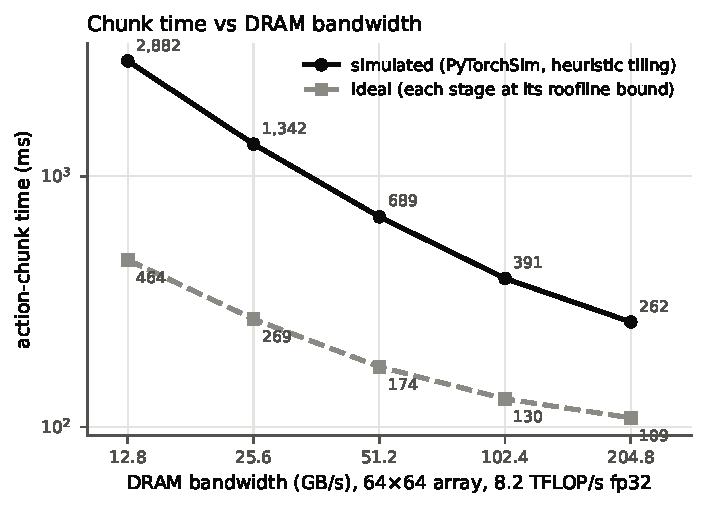
\includegraphics[width=0.5\textwidth]{p1/bandwidth_time.pdf}\\[0.5em]
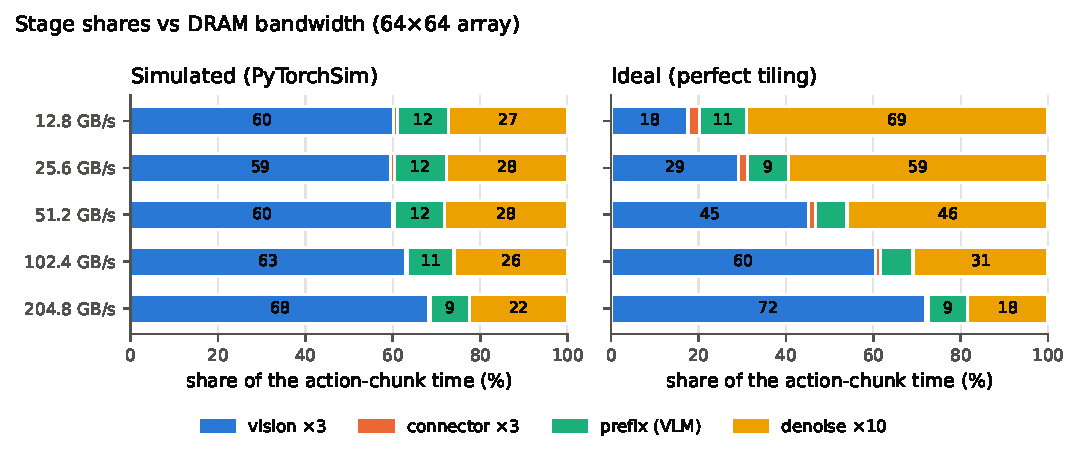
\includegraphics[width=\textwidth]{p1/bandwidth_shares.pdf}
\caption{DRAM-bandwidth sweep on the $64\times64$ NPU: chunk time (top) and stage shares (bottom), simulated by PyTorchSim and ideal (\cref{eq:ideal}).}
\label{fig:bw-sweep}
\vspace{1.5em}
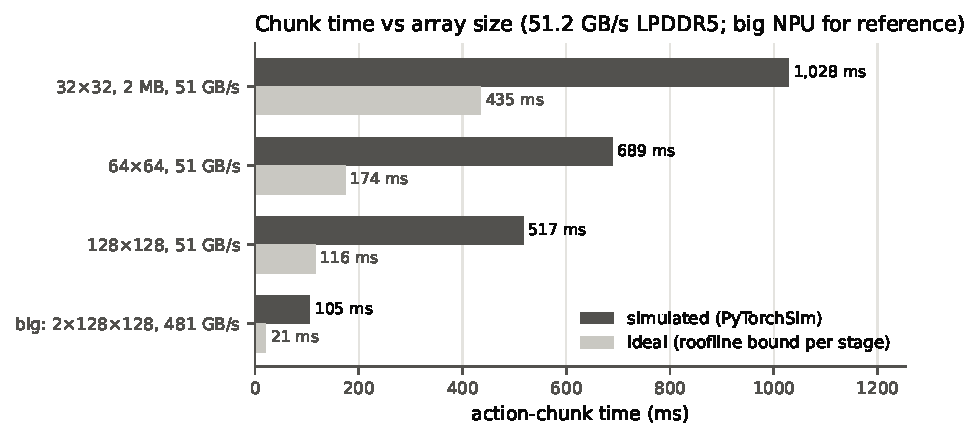
\includegraphics[width=0.55\textwidth]{p1/array_time.pdf}\\[0.5em]
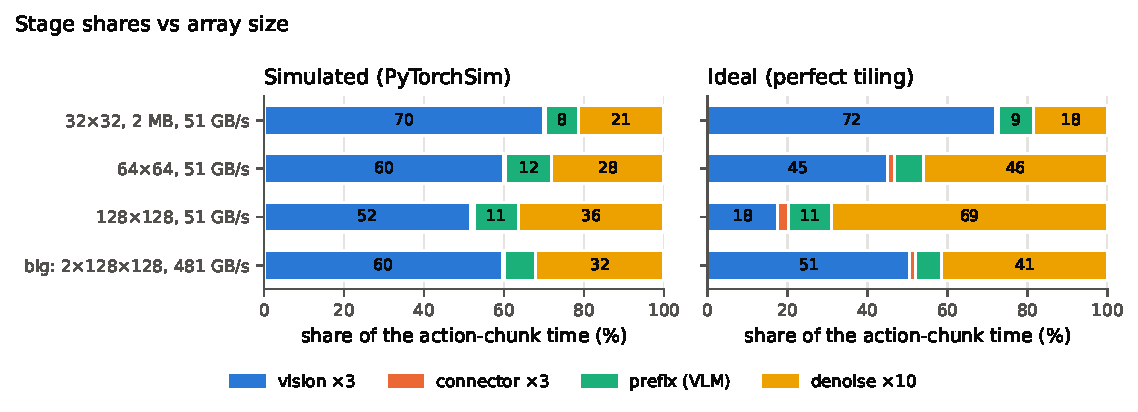
\includegraphics[width=\textwidth]{p1/array_shares.pdf}
\caption{Array-size sweep at 51.2~GB/s, with the big NPU for reference.}
\label{fig:array-sweep}
\end{figure}

\Cref{fig:bw-sweep} varies the DRAM bandwidth at fixed compute. Below about 100~GB/s the simulated NPU is bandwidth-bound end to end: halving the bandwidth doubles the chunk time (2882, 1343 and 689~ms at 12.8, 25.6 and 51.2~GB/s), with every stage at 77--84\% of the DRAM peak. The simulated stage shares therefore follow DRAM traffic and stay close to 60\% vision at every bandwidth.

The ideal model gives the opposite picture, and one that depends strongly on bandwidth. At 12.8~GB/s the denoise loop is \textbf{69\%} of the chunk, because the $\sim$400~MB of fp32 expert weights are streamed again in each of the 10 steps; at 205~GB/s vision is 72\%. The action expert dominates only on an NPU with a high ridge point (much compute per byte of bandwidth), and only if the other stages move little more than their compulsory traffic; \cref{subsec:wl-attribution} tests the second condition with forced tiling.

At a fixed 51.2~GB/s (\cref{fig:array-sweep}), growing the array from $32\times32$ to $128\times128$ gives diminishing returns (1028, 689 and 517~ms): prefix and denoise stay pinned at the DRAM limit, so the simulated denoise share rises to 36\% on $128\times128$. Doubling the $32\times32$ scratchpad from 2 to 4~MB changes the traffic by only $-4\%$ and the time by $+2\%$, because the heuristic tile sizes follow the lane count rather than the scratchpad capacity.

\subsection{Where the time and the traffic go}
\label{subsec:wl-attribution}

\begin{figure}[tp]
\centering
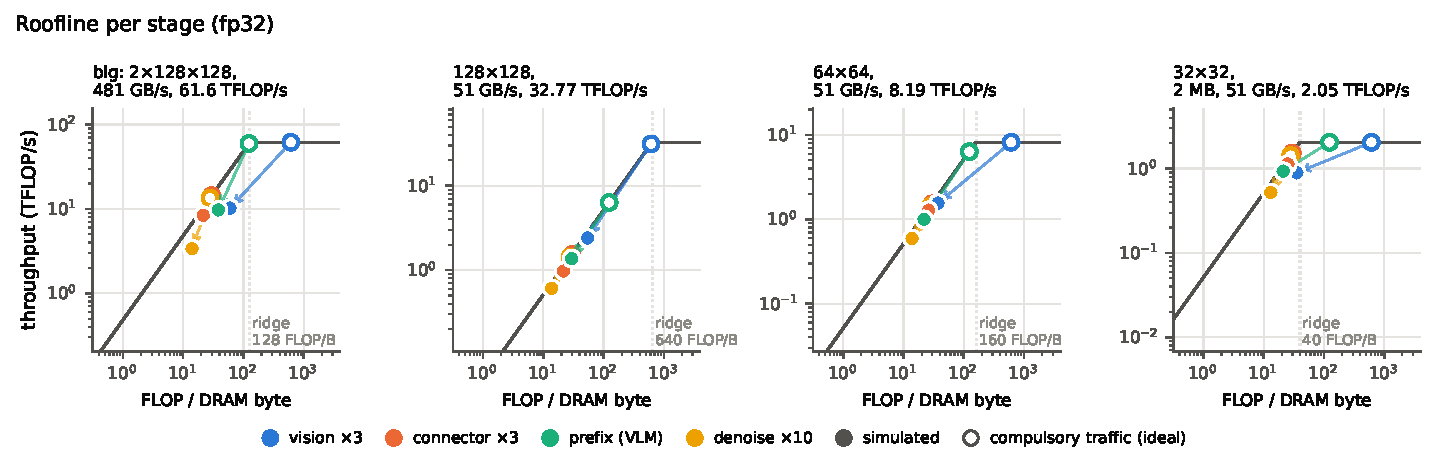
\includegraphics[width=\textwidth]{p1/roofline_stages.pdf}
\caption{Roofline per stage on four NPUs. Arrows go from the ideal point (compulsory traffic, hollow) to the simulated one (filled).}
\label{fig:roofline-stages}
\end{figure}

\Cref{fig:roofline-stages} shows the gap between simulated and ideal. Vision has an arithmetic intensity of 613~FLOP/B with compulsory traffic, but moves 10--17$\times$ that traffic, which pushes it from the compute roof onto the bandwidth slope. The prefix moves 3--7$\times$ its compulsory traffic, and the denoise step about $2\times$, since it is dominated by weights that must be read anyway. Over a whole chunk the simulated NPUs move 3.6--5.2$\times$ the compulsory traffic. The instruction-level replays (\cref{subsec:method-attribution}) show where this time and traffic go.

\begin{figure}[p]
\centering
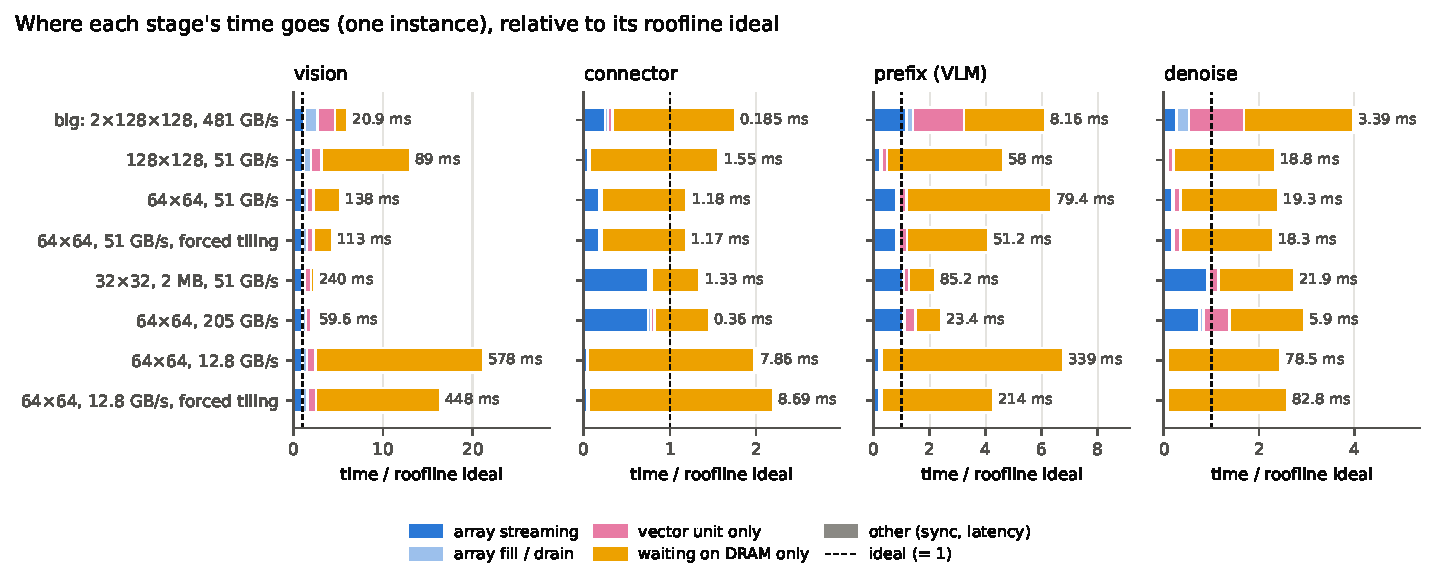
\includegraphics[width=\textwidth]{p1/attribution_time.pdf}
\caption{Time of one instance of each stage, relative to its roofline ideal (dashed line), from the instruction-level replays (\cref{subsec:method-attribution}).}
\label{fig:attr-time}
\vspace{1.5em}
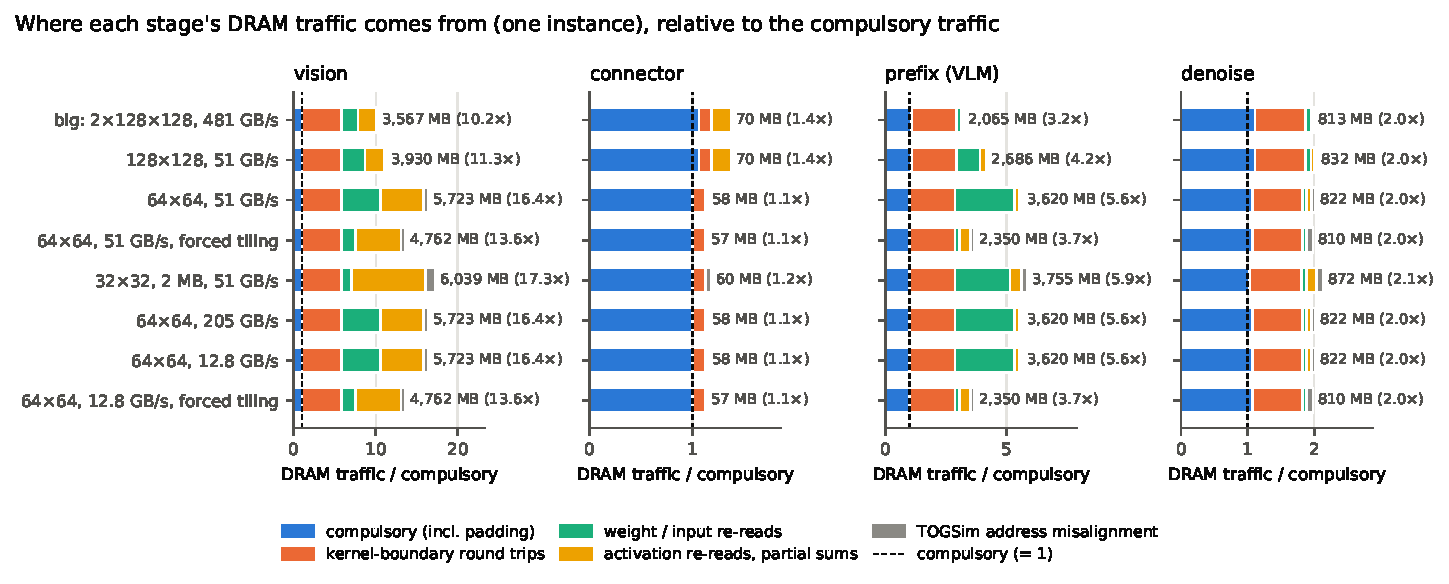
\includegraphics[width=\textwidth]{p1/attribution_traffic.pdf}
\caption{DRAM traffic of one instance of each stage by cause, relative to the compulsory traffic.}
\label{fig:attr-traffic}
\vspace{1.5em}
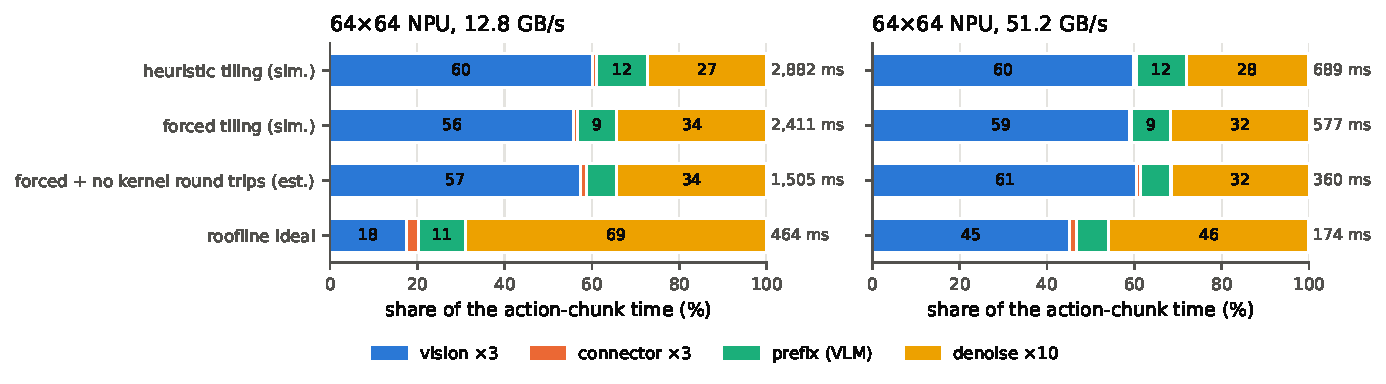
\includegraphics[width=\textwidth]{p1/scenarios.pdf}
\caption{Stage shares of the chunk on the $64\times64$ NPU: heuristic and forced tiling (simulated), forced tiling without kernel-boundary round trips (estimate) and the roofline ideal.}
\label{fig:scenarios}
\end{figure}

\Cref{fig:attr-time} shows that the array is never the bottleneck. While it streams, it executes exactly the ideal FLOPs plus the padding of the dimensions to the lane count: $1.00$--$1.07\times$ on $64\times64$ (720 padded to 768, 241 to 256), about $1.2\times$ on 128 lanes, and $1.3\times$ for the expert on $32\times32$ ($M=50$ padded to 64). The time is lost waiting: on the $64\times64$ NPU at 51.2~GB/s the stages wait on DRAM alone for 58--86\% of their time. On vision, $5.3\times$ its ideal, the array streams for $1\times$, unhidden fill/drain adds $0.5\times$, vector-only work $0.7\times$ and DRAM waits $3.1\times$.

\Cref{fig:attr-traffic} attributes the extra traffic. On $64\times64$, vision's $16\times$ comes from the MLP weights being re-read once per 128-row tile of the 1024 tokens (1.8~GB), from the flash-attention template re-reading K and V once per 64-row query tile (1.2~GB), from activations re-read per output tile, and from round trips between unfused kernels. The prefix's $5.6\times$ is mostly the MLP weights read four times (the heuristic chooses 64-row tiles of the 241 tokens) and round trips. The denoise step has no tiling waste at all: every weight is read once, and its extra traffic is the round trips between its many small kernels (37\%) plus the padding of 720 to 768 (+14\% on the weights).

Forced tiling (\cref{subsec:method-attribution}) confirms the attribution. At 51.2~GB/s it speeds up the prefix by 35\% and vision by 18\%, but the denoise step by only 5\%. Removing the round-trip bytes at the achieved bandwidth (an estimate of keeping each kernel's output on chip, which TOGSim cannot simulate) would bring the denoise step from 18.3 to 11.4~ms, against an ideal of 8.0~ms; the remainder is weight streaming at about 80\% of the DRAM peak. Even so, the denoise share reaches only 34\% at 12.8~GB/s (\cref{fig:scenarios}), against 69\% in the ideal model: vision still moves $13.6\times$ its compulsory traffic, because a 4~MB scratchpad holds only 256--512 of its 1024 token rows next to a weight tile, and because the flash-attention template fixes the query tile at the lane count. The action expert therefore dominates an NPU with a high ridge point only if vision runs close to its compulsory traffic, which takes on-chip memory sized for its activations, a K/V-resident attention tiling and fused element-wise kernels.

\subsection{How the stages respond to the hardware}
\label{subsec:wl-response}

The stages are different workloads (\cref{tab:stages}), so the same hardware change acts on them differently.

\begin{dashlist}
  \item \textbf{Bandwidth} shortens every DRAM wait but removes no byte. Ideally it speeds up only the memory-bound stages: the denoise step and the connector on every NPU, and the prefix above a ridge point of 124~FLOP/B. In simulation it also speeds up vision, which its extra traffic made memory-bound: 578, 138 and 60~ms at 12.8, 51.2 and 205~GB/s. At 205~GB/s vision's remaining loss is vector-only time and array fill/drain.
  \item \textbf{Array size} helps only compute-bound work: ideally vision and, on high-bandwidth NPUs, the prefix; never the denoise step.
  \item \textbf{The ideal split depends only on the ridge point} (peak over bandwidth), not on the size of the NPU: NPUs with the same ridge point give the same split (18\% at 40~FLOP/B, 41--46\% at 128--160, 69\% at 640, e.g.\ $64{\times}64$ at 12.8~GB/s and $128{\times}128$ at 51.2~GB/s). A large array and a low bandwidth are the same condition. The denoise share saturates at 69\%, its part of the compulsory bytes of a chunk (4.1 of 5.9~GB), which it reaches when every stage is memory-bound.
  \item \textbf{Scratchpad.} Vision needs capacity: one activation is 3~MB and the MLP hidden one 12.6~MB, and a GEMM tile holds an input, a weight and an output block, double-buffered. With the traffic-minimising tiles of \cref{subsec:wl-attribution}, its GEMMs still move 1.3--1.6$\times$ their minimum traffic at 16~MB and reach it only at about 64~MB. The 16~MB big NPU moves $10\times$ the compulsory traffic for three reasons, none of them a lack of capacity alone: the heuristic tiles read the MLP weights 4 times (256-row tiles of the 1024 tokens), the flash-attention template reads K and V 8 times (its query tile is fixed at the 128 lanes), and every kernel's output makes a DRAM round trip. The mapping matters as much as the size. The denoise step needs almost none: with forced tiling its GEMMs already move the minimum traffic on 4~MB, and fusing all its kernels needs less than 1~MB. Its cost is the ${\approx}400$~MB of weights read in every step. These reads are compulsory, because the 10 steps are sequential and no edge scratchpad holds the weights; only bandwidth or fewer bytes per weight (bf16 $2\times$, int8 $4\times$) reduce them.
  \item \textbf{Fusion} (no kernel-boundary round trips) is cheap for the expert and the prefix, whose intermediates are below 3~MB. For vision it competes with the weight tiles for the same scratchpad.
\end{dashlist}

\subsection{Cross-check with SCALE-Sim}
\label{subsec:wl-scalesim}

\begin{figure}[tp]
\centering
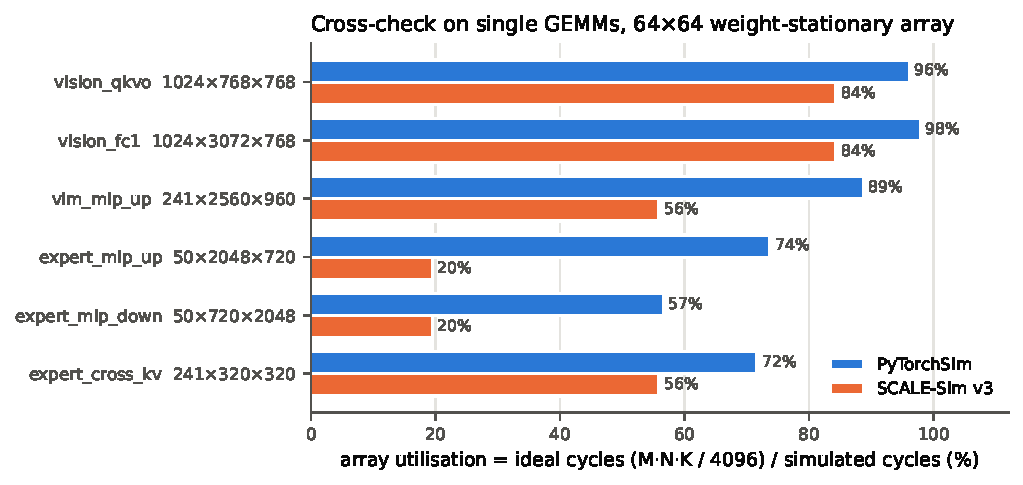
\includegraphics[width=0.8\textwidth]{p1/scalesim_check.pdf}
\caption{Array utilisation on single GEMMs, $64\times64$ weight-stationary array, both simulators compute-bound.}
\label{fig:scalesim}
\end{figure}

On the large vision GEMMs PyTorchSim and SCALE-Sim agree within about 15\% (\cref{fig:scalesim}). On the thin GEMMs ($M = 50$ for the expert, $M = 241$ for the VLM) SCALE-Sim is up to $3.8\times$ slower. The difference is how weight tiles are loaded. PyTorchSim double-buffers them, loading the next $64\times64$ weight tile while the current one computes. SCALE-Sim's weight-stationary model instead serialises weight load, fill and drain for every fold. Before SCALE-Sim is used to explore the expert's design space, that per-fold gap must be removed or accounted for.

\subsection{Discussion}
\label{subsec:wl-discussion}

\begin{dashlist}
  \item \textbf{Stage balance depends on the compiler as much as on the hardware.} With PyTorchSim's heuristic tiling, vision dominates (52--70\%) on every simulated NPU, and still 56--59\% with traffic-minimising GEMM tiles. With perfect tiling, the dominant stage is set by the ridge point: vision on NPUs with little compute per byte of bandwidth, the action expert's denoise loop (up to 69\%) on NPUs with much. What separates the two is vision's traffic, set by the scratchpad size and the attention tiling.
  \item \textbf{The array is not the bottleneck.} While streaming it runs at the ideal rate up to padding; the time is lost waiting on DRAM and on the vector unit.
  \item \textbf{The denoise loop is a weight-streaming problem.} At batch 1 it re-reads the expert weights in each of its 10 steps, about 69\% of the compulsory traffic of a chunk. Tiling cannot help it; removing the round trips between its small kernels is worth about a third of its time. Keeping the weights on chip across steps would need about 400~MB, out of reach for an edge NPU; reduced precision (bf16 halves the bytes, int8 quarters them) and caching the cross-attention K/V of the fixed prefix act directly on this term.
  \item \textbf{The vision encoder stresses compute and the vector unit.} Its fused attention is bound by the vector unit, which scales with the array in PyTorchSim, so attention is the critical part of vision on small arrays.
  \item \textbf{The stages want different resources} (\cref{subsec:wl-response}). Vision wants compute, a vector unit that keeps up with the array, and on-chip capacity of tens of MB with a mapper that uses it. The action expert wants bandwidth and fewer bytes per weight; a larger scratchpad does not help it. These opposite demands, and the ridge point that sets the balance between them, are the starting point for the design-space exploration of the next part (array size, scratchpad size, bandwidth, precision, varied one at a time with SCALE-Sim) and for the question of a heterogeneous edge NPU.
\end{dashlist}
